\documentclass[letterpaper,11pt]{article}

\usepackage{latexsym}
\usepackage[empty]{fullpage}
\usepackage{titlesec}
\usepackage{marvosym}
\usepackage[usenames,dvipsnames]{color}
\usepackage{verbatim}
\usepackage{enumitem}
\usepackage[hidelinks]{hyperref}
\usepackage{fancyhdr}
\usepackage[english]{babel}
\usepackage{tabularx}
\usepackage{fontawesome5}
\usepackage{multicol}
\setlength{\multicolsep}{-3.0pt}
\setlength{\columnsep}{-1pt}
\input{glyphtounicode}

%new packages

\usepackage{fontenc}
\usepackage{amsmath}
\usepackage{amssymb}
\usepackage{graphicx}



%----------FONT OPTIONS----------

\pagestyle{fancy}
\fancyhf{} % clear all header and footer fields
\fancyfoot{}
\renewcommand{\headrulewidth}{0pt}
\renewcommand{\footrulewidth}{0pt}

% Adjust margins
\addtolength{\oddsidemargin}{-0.6in}
\addtolength{\evensidemargin}{-0.5in}
\addtolength{\textwidth}{1.19in}
\addtolength{\topmargin}{-.7in}
\addtolength{\textheight}{1.4in}

\urlstyle{same}

\raggedbottom
\raggedright
\setlength{\tabcolsep}{0in}

% Sections formatting
\titleformat{\section}{
  \vspace{-4pt}\scshape\raggedright\large\bfseries
}{}{0em}{}[\color{black}\titlerule \vspace{-5pt}]



% Ensure that generate pdf is machine readable/ATS parsable
\pdfgentounicode=1

%-------------------------
% Custom commands
\newcommand{\resumeItem}[1]{
  \item\small{
    {#1 \vspace{-2pt}}
  }
}

\newcommand{\classesList}[4]{
    \item\small{
        {#1 #2 #3 #4 \vspace{-2pt}}
  }
}

\newcommand{\resumeSubheading}[4]{
  \vspace{-2pt}\item
    \begin{tabular*}{1.0\textwidth}[t]{l@{\extracolsep{\fill}}r}
      \textbf{#1} & \textbf{\small #2} \\
      \textit{\small#3} & \textit{\small #4} \\
    \end{tabular*}\vspace{-7pt}
}

\newcommand{\resumeSubSubheading}[2]{
    \item
    \begin{tabular*}{0.97\textwidth}{l@{\extracolsep{\fill}}r}
      \textit{\small#1} & \textit{\small #2} \\
    \end{tabular*}\vspace{-7pt}
}

\newcommand{\resumeProjectHeading}[2]{
    \item
    \begin{tabular*}{1.001\textwidth}{l@{\extracolsep{\fill}}r}
      \small#1 & \textbf{\small #2}\\
    \end{tabular*}\vspace{-7pt}
}


\newcommand{\resumeSubItem}[1]{\resumeItem{#1}\vspace{-4pt}}

\renewcommand\labelitemi{$\vcenter{\hbox{\tiny$\bullet$}}$}
\renewcommand\labelitemii{$\vcenter{\hbox{\tiny$\bullet$}}$}

\newcommand{\resumeSubHeadingListStart}{\begin{itemize}[leftmargin=0.0in, label={}]}
\newcommand{\resumeSubHeadingListEnd}{\end{itemize}}
\newcommand{\resumeItemListStart}{\begin{itemize}}
\newcommand{\resumeItemListEnd}{\end{itemize}\vspace{-5pt}}

\begin{document}
\fontfamily{cmr}\selectfont
\begin{center}
\parbox{3.0cm}{%
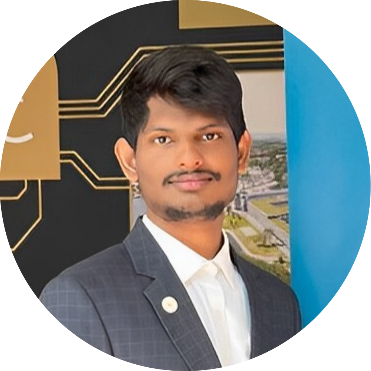
\includegraphics[width=2.7cm,clip]{images/resume_pic_m.png}}
\parbox{\dimexpr\linewidth-3.8cm\relax}{
\vspace{-20pt}
\begin{tabularx}{\linewidth}{L r} \\
    {\Huge \scshape  Venkata Sai Yakkshit Reddy Asodi}~
    \href{https://www.cedzlabs.com/yakkshit}{\vspace{1pt}}\\
      Berlin, Germany. \\ \vspace{1pt}
     \small \raisebox{-0.1\height}\faPhone\ +91 8179936156 ~ \href{mailto:saiyakkshit2001@gmail.com}{\raisebox{-0.2\height}\faEnvelope\  {saiyakkshit2001@gmail.com}} ~ 
    \href{https://linkedin.com/in/yakkshit/}{\raisebox{-0.2\height}\faLinkedin\ {yakkshit}}  ~
    \href{https://yakkshit.com/}{\raisebox{-0.2\height}\faGlobe\ {yakkshit.com}}  ~
    \href{https://github.com/yakkshit}{\raisebox{-0.2\height}\faGithub{ yakkshit}}
    \vspace{-8pt}
\end{tabularx}
}
\end{center}

\vspace{-23pt}
\section{Summary}
Full Stack Engineer with 3+ years of experience building engaging, interactive web applications. Skilled in JavaScript, React, and Node.js, with a passion for AI-driven solutions and improving educational tools. Experienced in microservices architecture and deploying scalable applications on AWS.

\section{Technical Skills}
\begin{itemize}[leftmargin=0.15in, label={}]
\small{\item{
\textbf{Frameworks: }{React, Next.js, Node.js} \\
\textbf{Languages: }{JavaScript, TypeScript, GraphQL, Python} \\
\textbf{Tools: }{AWS, Docker, Git, GraphQL APIs, Microservices, RESTful APIs, Vercel} \\
\textbf{Deployment: }{AWS, RDS, Neon, Microservices.}\\
}}
\end{itemize}

\section{Experience}

\resumeSubHeadingListStart
\resumeSubheading
{\large Circleup AG}{December 2023 -- July 2024}
  {Lead Full Stack Engineer}{Zurich, Switzerland}
\vspace{-5pt}
\begin{itemize}[leftmargin=0.15in, label={}]
\item Developed features for interactive learning tools using React and Node.js.
\item Integrated APIs for LLM-based personalized learning.
\item Optimized the app for scalability, performance, and AI-driven educational tools.
\end{itemize}

\resumeSubheading
{\large Cedzlabs}{March 2023 -- July 2024}
  {Full Stack Engineer}{India}
\vspace{-5pt}
\begin{itemize}[leftmargin=0.15in, label={}]
\item Built dynamic web applications using React and Next.js.
\item Integrated GraphQL APIs and optimized deployment on AWS and Vercel.
\end{itemize}

\section{Projects}
\resumeProjectHeading
{\textbf{AI Resume Tuner} | \emph{Azure Cloud, Next.js, LLMs, RAG}}{August 2023}
\begin{itemize}[leftmargin=0.15in, label={}]
\item Developed a tool for generating personalized resumes using AI and LLMs, with backend APIs hosted on Azure Cloud.
\end{itemize}

\resumeProjectHeading
{\textbf{Portfolio Website} | \emph{NextJS, AWS}}{January 2023}
\begin{itemize}[leftmargin=0.15in, label={}]
\item Created a portfolio website with secure file encryption and scalable design using NextJS and AWS.
\end{itemize}

\section{Achievements}
\begin{itemize}[leftmargin=0.15in, label={}]
\item Integrated AI-assisted features for adaptive learning systems in education.
\item Contributed to open-source projects and active in tech meetups.
\item Proven leadership in managing teams and delivering high-quality web solutions.
\end{itemize}

\section*{Languages}
Telugu - Native | English - Fluent | Hindi - Fluent | German - Elementary | Swedish - Elementary

\end{document}